\documentclass[xcolor=dvipsnames]{beamer}
% If you want to print these slide as a handout, use the following instead:
% \documentclass[handout,xcolor=dvipsnames]{beamer}


\usepackage{xcolor}
\usepackage{hyperref}
\usepackage{lmodern}
\usepackage[english]{babel}
\usepackage[utf8]{inputenc}
%\usepackage{times}
\usepackage{caption}
%\usepackage{subcaption}
%\captionsetup{compatibility=false}
\usepackage{amsmath}
\usepackage{epstopdf}
\usepackage{listings}


\mode<presentation>
{
    \usetheme{Malmoe}      % or try 'Frankfurt'
    \usecolortheme[named=OliveGreen]{structure}
    \usefonttheme{structurebold}
    \setbeamercovered{invisible}  % or transparent
}


\hypersetup
{
    unicode=true,
    pdfauthor={Ryan Henning}
}


\title[SVMs]
{Support Vector Machines}

\author
{Ryan Henning}

\institute
{
    Galvanize
}

\date
{June 2, 2016}


% If you have a file called "university-logo-filename.xxx", where xxx
% is a graphic format that can be processed by latex or pdflatex,
% resp., then you can add a logo as follows:
% \pgfdeclareimage[height=0.5cm]{university-logo}{university-logo-filename}
% \logo{\pgfuseimage{university-logo}}


\AtBeginSubsection[]
{
    \begin{frame}<beamer>{Outline}
        \tableofcontents[
            currentsection,
            currentsubsection,
            %hideothersubsections,
            subsectionstyle=show/shaded,
            %sectionstyle=show/shaded,
        ]
    \end{frame}
}


% If you wish to uncover everything in a step-wise fashion, uncomment
% the following command:
% \beamerdefaultoverlayspecification{<+->}


\begin{document}

\begin{frame}
    \titlepage
\end{frame}


\begin{frame}{Objectives}{Support Vector Machines (SVMs) Lecture}
    \begin{enumerate}
        \item Gain an intuition about the {\em purpose} and {\em power} of SVMs.
        \item<2-> Explore (some) of the mathematics behind SVMs.
        \item<3-> Supercharge SVMs with kernels and soft margins.
        \item<4-> Gain an intuition about the Bias-Variance tradeoff while using SVMs.
    \end{enumerate}
\end{frame}

\begin{frame}{Support Vector Machines}{A rough history}
    \uncover<2->{
        \vspace{1em}
        {\bf Maximum Margin Classifier:} (morning lecture)\\
        1963: Vapnik, Chervonenkis\\
        \vspace{2em}
    }
    \uncover<3->{
        {\bf Soft Margins and the ``Kernel Trick'':} (afternoon lecture)\\
        1992-1995: Vapnik, Boser, Guyon, Cortes\\
    }
    \uncover<4->{
        \alert{This is the modern Support Vector Machine (SVM).}\\
    }
\end{frame}


\section{Review}

\subsection{Supervised Learning}

\begin{frame}{Supervised Learning}
    \textbf{High level:} \uncover<1-1>{\alert{What is supervised learning?}}\\
    \vspace{2em}
    \uncover<2->{
        Learn an unknown function from a set of {\bf labeled} training data.
    }
    \vspace{0.5em}
    \begin{itemize}
        \item<3-> Our training data is limited and finite. A useful algorithm must generalize well to ``unseen'' data.
        \item<4-> Example: Children learning colors.
        \item<5-> Support Vector Machines (SVMs) are a {\em supervised} learning algorithm.
    \end{itemize}
\end{frame}

\subsection{Notation}

\begin{frame}{Notation}
    \textbf{Goal:}\\
    \vspace{0.5em}
    Learn a model of a function $F:X \rightarrow Y$ from a training set $D$.\\
    \vspace{2em}
    \uncover<2->{
        $D = \{(x^{(1)}, y^{(1)}), \dots, (x^{(m)}, y^{(m)})\}$, where
        \vspace{1em}
        \begin{itemize}
            \item $x^{(j)} \in X$ is often called the ``input''.
            \item $y^{(j)} \in Y$ is often called the ``label'' or ``target''.
        \end{itemize}
    }
\end{frame}

\begin{frame}{Notation (cont.)}
    $F:X \rightarrow Y$
    \vspace{1em}
    \begin{itemize}
        \item Often, $X = \mathbb{R}^n$
        \item Often, $Y$ is a finite set (i.e. a classification task)
    \end{itemize}
    \vspace{2em}
    \uncover<2->{
        We want our learned model to {\em generalize} well.\\
    }
    \uncover<2-2>{
        \alert{Explain the concept of ``generalization error``.}\\
    }
    \uncover<3->{
        \vspace{1em}
        Generalization error is a measure of the model's performance on all possible ``unseen'' data.
    }
\end{frame}

\subsection{Hyperplanes}

\begin{frame}{Dimensions}{Basic stuff, I know.}
    \vspace{1em}
    \begin{center}
        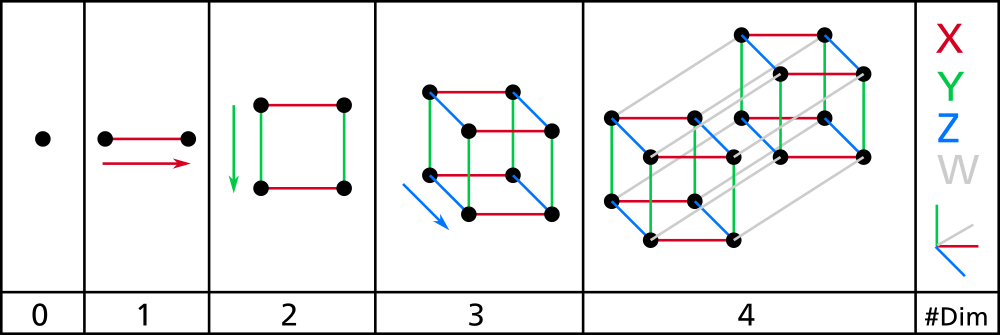
\includegraphics[width=\textwidth]{figs/Dimension_levels.png}\\
    \end{center}
    \footnotetext[1]{By NerdBoy1392 (Own work) [CC BY-SA 3.0 (http://creativecommons.org/licenses/by-sa/3.0)], via Wikimedia Commons}
\end{frame}

\begin{frame}{1D}{How do you split this space?}
    \begin{center}
        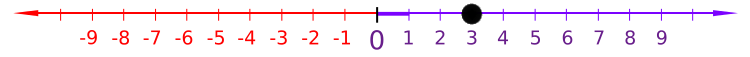
\includegraphics[width=0.6\textwidth]{figs/Number-line.png}\\
        \vspace{2em}
        \uncover<2->{
            Split a line (1D) with a point (0D).
        }
    \end{center}
    \footnotetext[1]{By HakunamentaMathsIsFun at en.wikipedia [CC0], from Wikimedia Commons, Public Domain}
\end{frame}

\begin{frame}{2D}{How do you split this space?}
    \begin{center}
        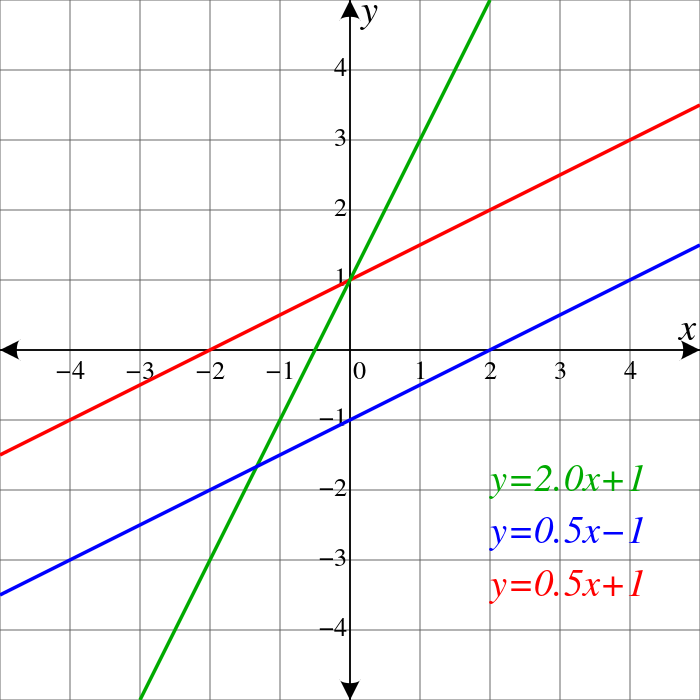
\includegraphics[width=0.3\textwidth]{figs/Linear-functions.png}\\
        \vspace{0.5em}
        \uncover<2->{
            Split a plane (2D) with a line (1D).
        }
    \end{center}
    \footnotetext[1]{By ElectroKid (talk • contribs). Original: HiTe. (Modification from the original work.) [CC BY-SA 1.0 (http://creativecommons.org/licenses/by-sa/1.0)], via Wikimedia Commons}
\end{frame}

\begin{frame}{3D}{How do you split this space?}
    \begin{center}
        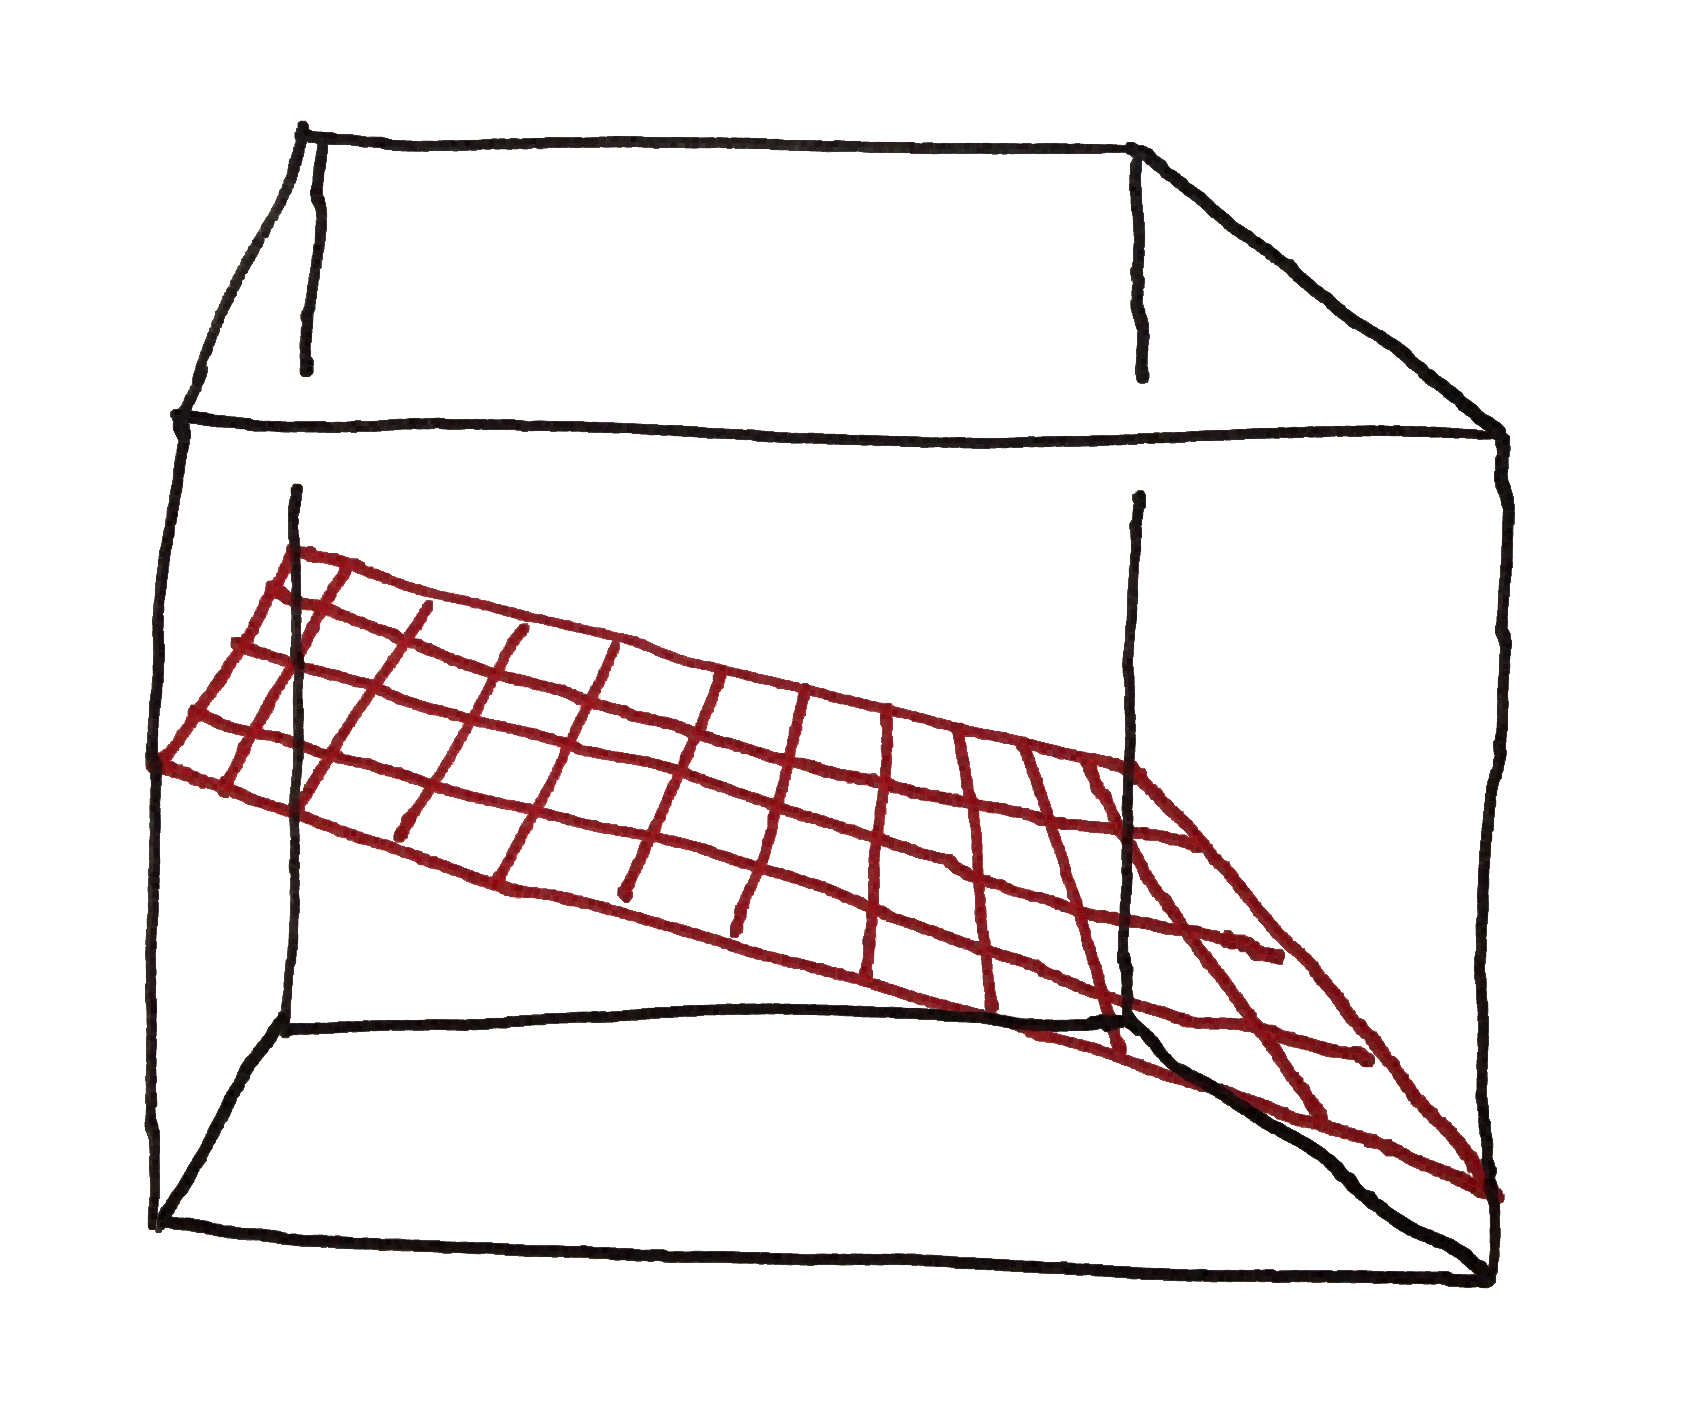
\includegraphics[width=0.3\textwidth]{figs/3d_sep_mine.png}\\
        \vspace{0.5em}
        \uncover<2->{
            Split space (3D) with a plane (2D).
        }
    \end{center}
    \vspace{2em}
\end{frame}

\begin{frame}{4D, 5D, etc...}{Hard to visualize... :/}
    In general, an $n$-dimensional space can be separated by an $(n-1)$-dimensional {\em hyperplane}.\\
    \vspace{2em}
    \uncover<2->{
        In an $n$-dimensional space any hyperplane can be defined by $w \in \mathbb{R}^n$ and $b \in \mathbb{R}$. The hyperplane includes all $x \in \mathbb{R}^n$ where:\\
        $$w_0 x_0 + w_1 x_1 + ... + w_{n-1} x_{n-1} - b = 0$$
    }
    \uncover<3->{
        usually written:
        $$w \cdotp x - b = 0$$
    }
\end{frame}

\begin{frame}{How to interpret $w$ and $b$}
    So, $w$ and $b$ define a hyperplane. Is there an interpretation of $w$ and $b$ that can help us visualize this hyperplane?
    \vspace{1em}
    \begin{itemize}
        \item<2-> $\frac{w}{||w||}$ is the hyperplane's normal vector.
        \item<3-> $\frac{b}{||w||}$ is the hyperplane's distance from the origin.
    \end{itemize}
    \vspace{2em}
\end{frame}

\begin{frame}{Example in 2D}
    \begin{center}
        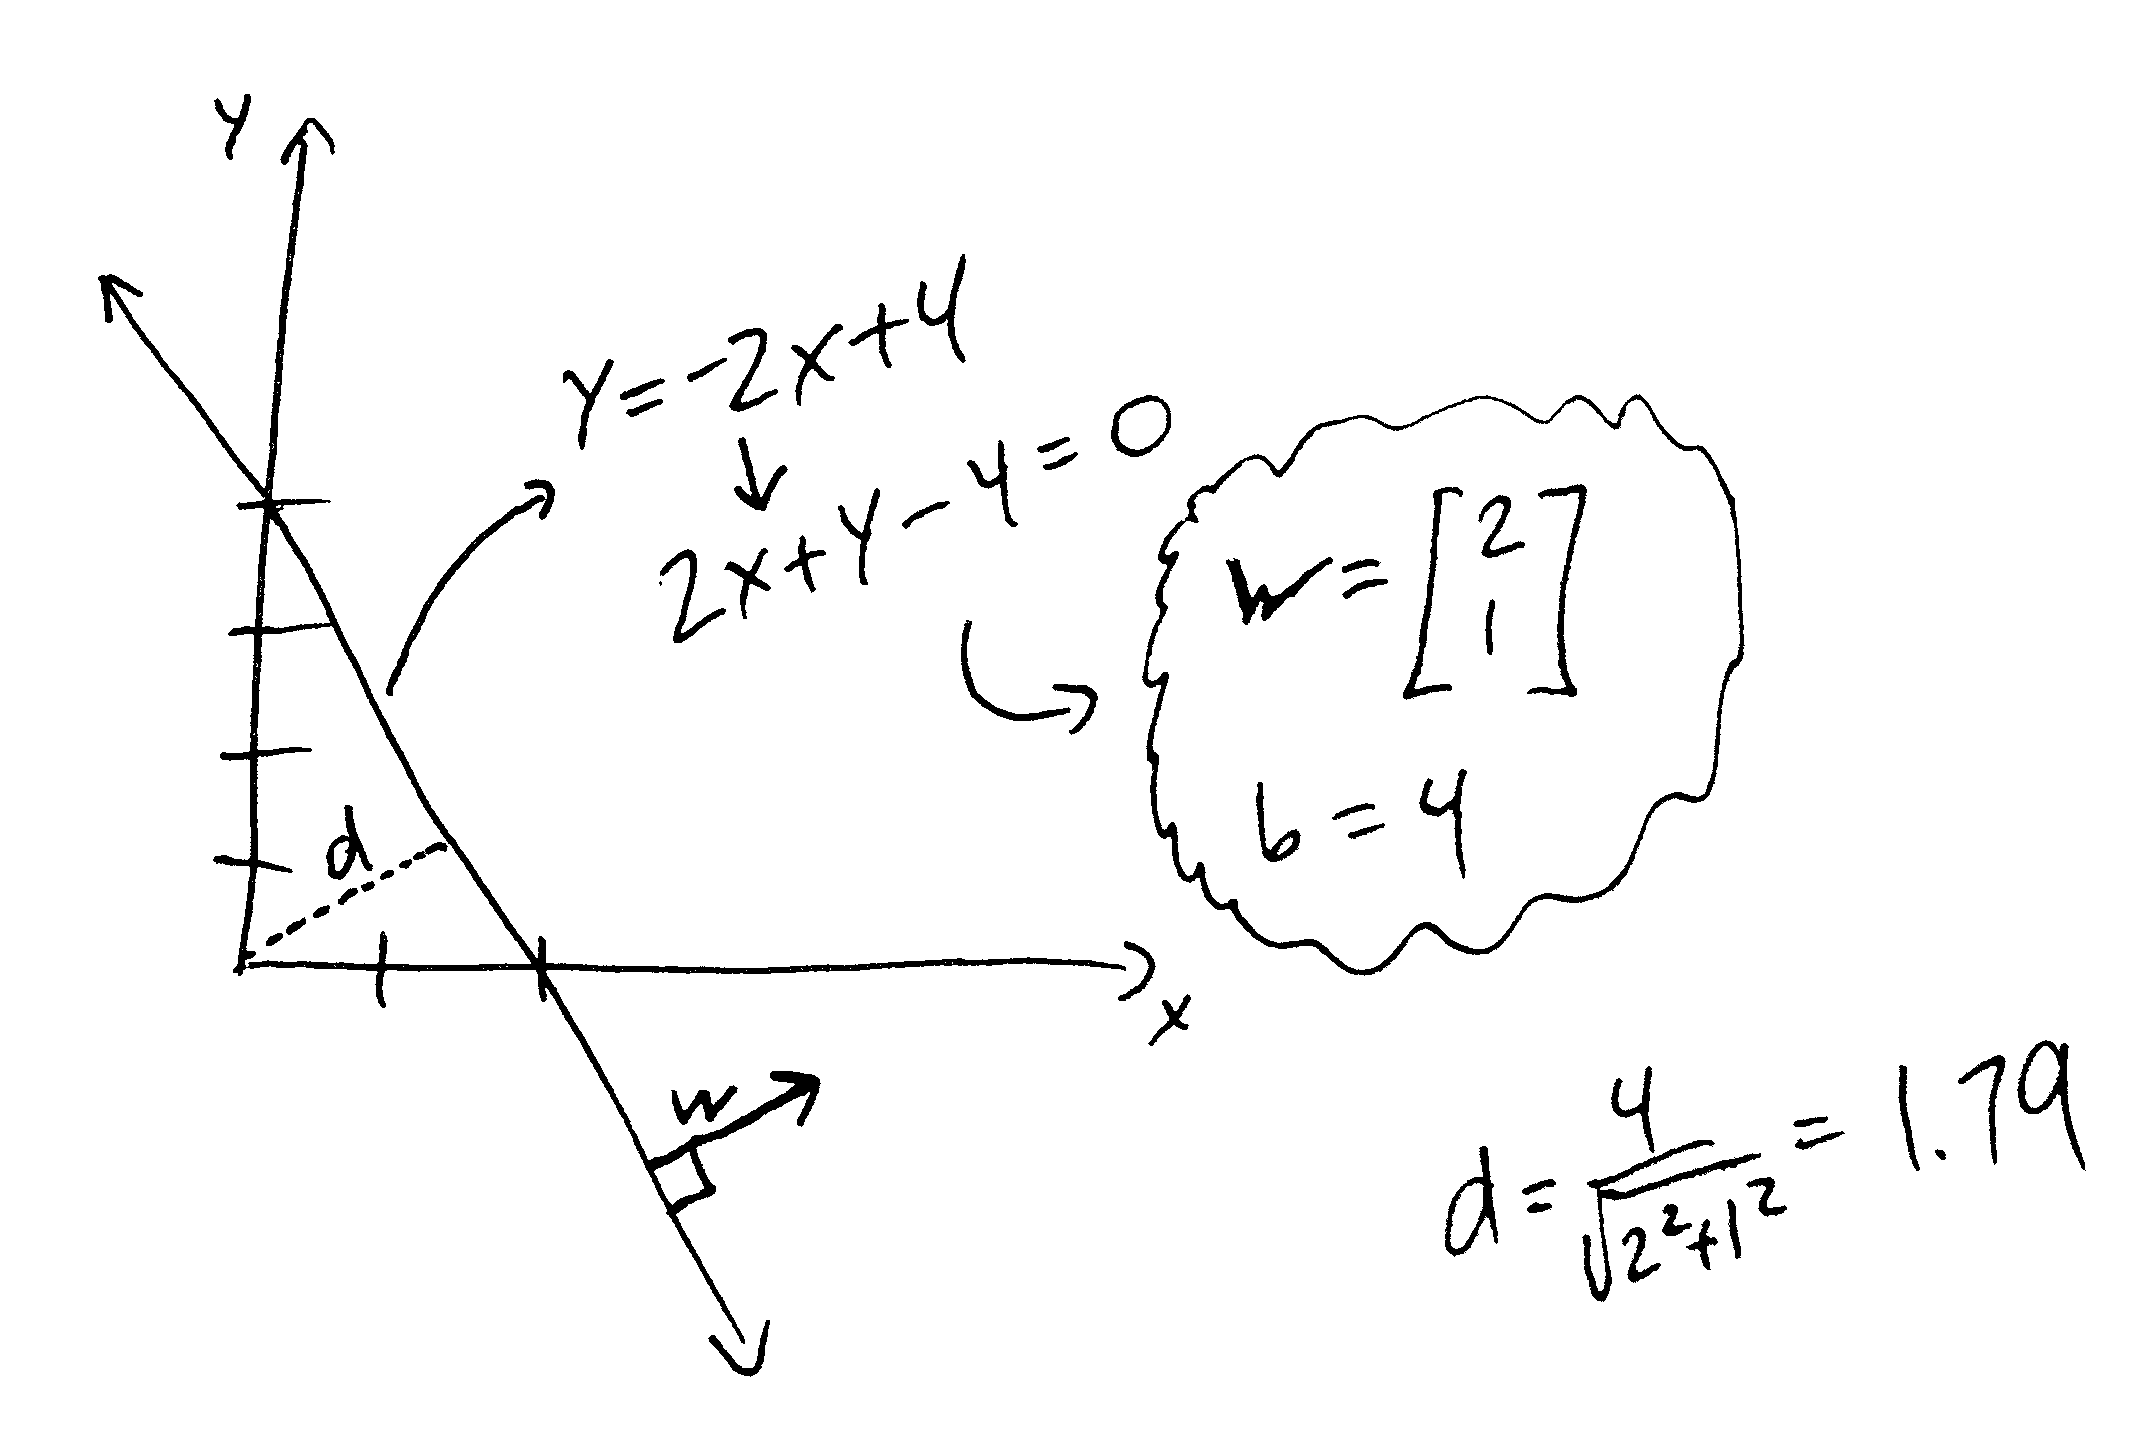
\includegraphics[width=0.7\textwidth]{figs/2d_hyper_example.png}
    \end{center}
\end{frame}

\section{Motivation}

\subsection{Binary Classification}

\begin{frame}{Binary Classification}{A supervised learning problem}
    Recall, we're trying to learn $F:X \rightarrow Y$.\\
    \vspace{0.5em}
    \begin{itemize}
        \item Let, $X = \mathbb{R}^n$
        \item For binary classification, $Y = \{-1, 1\}$\\
            \uncover<2->{\alert{We're using -1 instead of 0 for future mathematical convenience.}}
    \end{itemize}
    \vspace{2em}
    \uncover<3->{
        Big idea: Let's have our model find a hyperplane that splits our $n$-dimensional data $X$ into the set where $y=-1$ and the set where $y=1$.
    }
\end{frame}

\begin{frame}{Binary Classification: Example}{How many ways can we use a hyperplane to classify this dataset correctly?}
    \begin{center}
        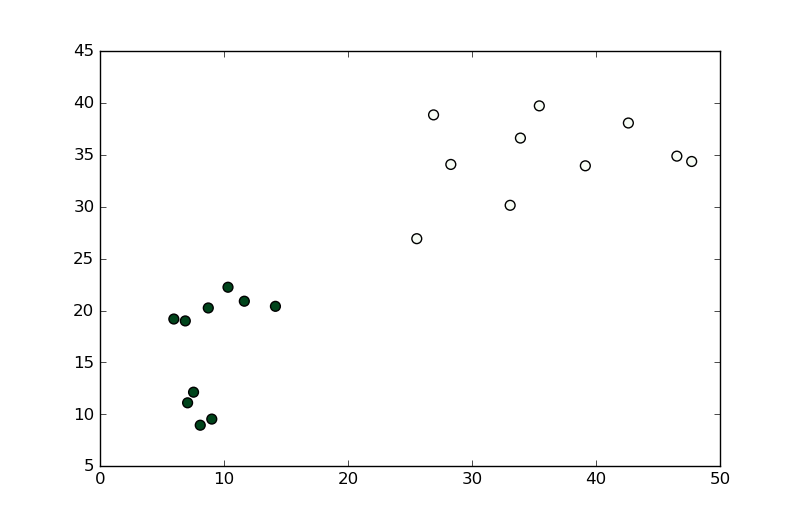
\includegraphics[width=0.7\textwidth]{figs/binclass_1.png}
    \end{center}
    $$X = \mathbb{R}^2$$
    $$Y = \{-1, 1\}$$
\end{frame}

\begin{frame}{Binary Classification: Example}{Two Example Solutions}
    \begin{columns}
        \begin{column}{0.5\textwidth}
            \begin{center}
                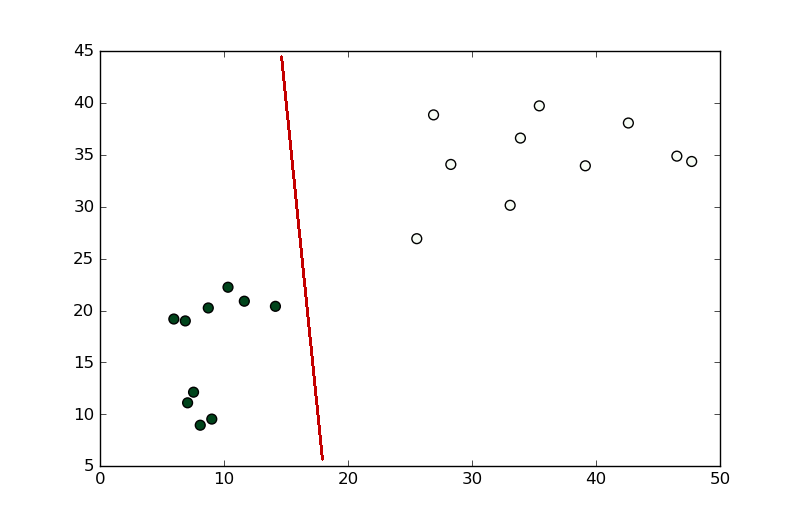
\includegraphics[width=\textwidth]{figs/binclass_2.png}
            \end{center}
        \end{column}
        \begin{column}{0.5\textwidth}
            \begin{center}
                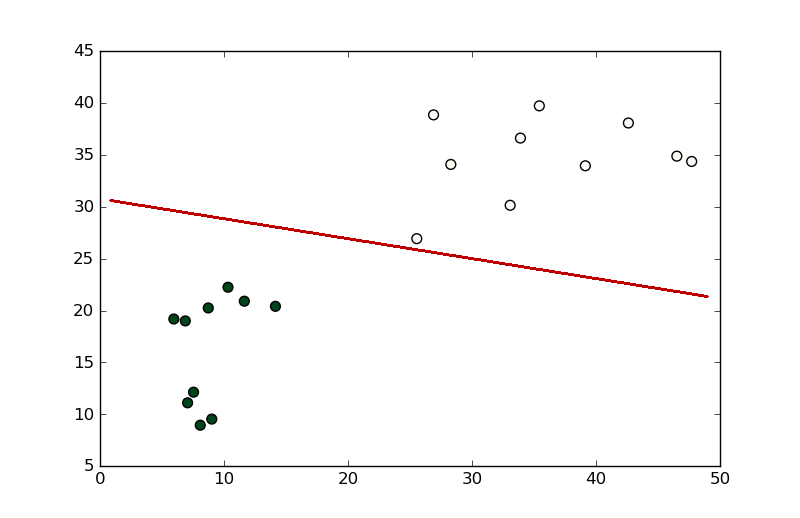
\includegraphics[width=\textwidth]{figs/binclass_3.png}
            \end{center}
        \end{column}
    \end{columns}
\end{frame}

\subsection{Margin}

\begin{frame}{Defining Margin}
    The distance from the hyperplane to the nearest training-data point.\\
    \uncover<2->{
        \begin{center}
            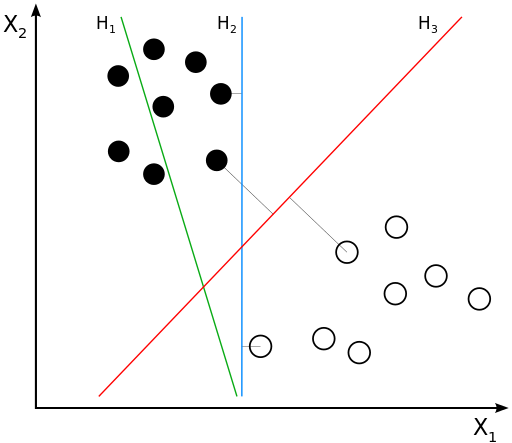
\includegraphics[width=0.5\textwidth]{figs/512px-Svm_separating_hyperplanes.png}
        \end{center}
    }
    \footnotetext[1]{By User:ZackWeinberg, based on PNG version by User:Cyc [CC BY-SA 3.0 (http://creativecommons.org/licenses/by-sa/3.0)], via Wikimedia Commons}
\end{frame}

\begin{frame}{Why Maximize the Margin?}
    Our goal is to train a model that generalizes to ``unseen'' data. \\
    \vspace{1em}
    \uncover<2->{Large margin means better generalization.}
    \vspace{1em}
    \begin{itemize}
        \item<3-> Intuitively, this makes sense (see previous slide)
        \item<4-> As margin increases, VC-dimension decreases, meaning variance decreases
    \end{itemize}
\end{frame}

\subsection{Maximum Margin Classifier}

\begin{frame}{Maximum Margin Classifier}{Goal}
    Goal: Calculate $w$ and $b$ of the hyperplane:
    $$w \cdotp x - b = 0$$
    \uncover<2->{
        ... such that the classes are split correctly and the margin is maximized.\\
    }
    \vspace{3em}
    \uncover<3->{
        First, some house cleaning: \alert{What happens to the hyperplane when we scale $w$ and $b$ by some factor $c$?}
    }
\end{frame}

\begin{frame}{Maximum Margin Classifier}{Setup}
    We need to define a ``canonical'' $w$ and $b$. This will help later.\\
    \vspace{1em}
    Let
    $$| w \cdotp x^{(i)} - b | = 1$$
    where $x^{(i)}$ is the closest point to the hyperplane.\\
    \vspace{2em}
    \uncover<2->{
        There will be a unique scaled $w$ and $b$ to achieve this.
    }
\end{frame}

\begin{frame}{Maximum Margin Classifier}{Margin}
    Now, if $x^{(i)}$ is the closest point to the hyperplane, then the distance from $x^{(i)}$ to the hyperplane is our margin. What is that distance?
    \vspace{1em}
    \begin{columns}
        \begin{column}{0.5\textwidth}
            \uncover<2->{
                $$\left| \frac{w}{||w||} \cdotp (x^{(i)}-x) \right| = d$$
            }
            \uncover<3->{
                $$\frac{| w \cdotp x^{(i)} - w \cdotp x |}{||w||} = d$$
            }
            \uncover<4->{
                $$\frac{| w \cdotp x^{(i)} - b - w \cdotp x + b |}{||w||} = d$$
            }
            \uncover<5->{
                $$\frac{1}{||w||} = d = margin$$
            }
        \end{column}
        \begin{column}{0.5\textwidth}
            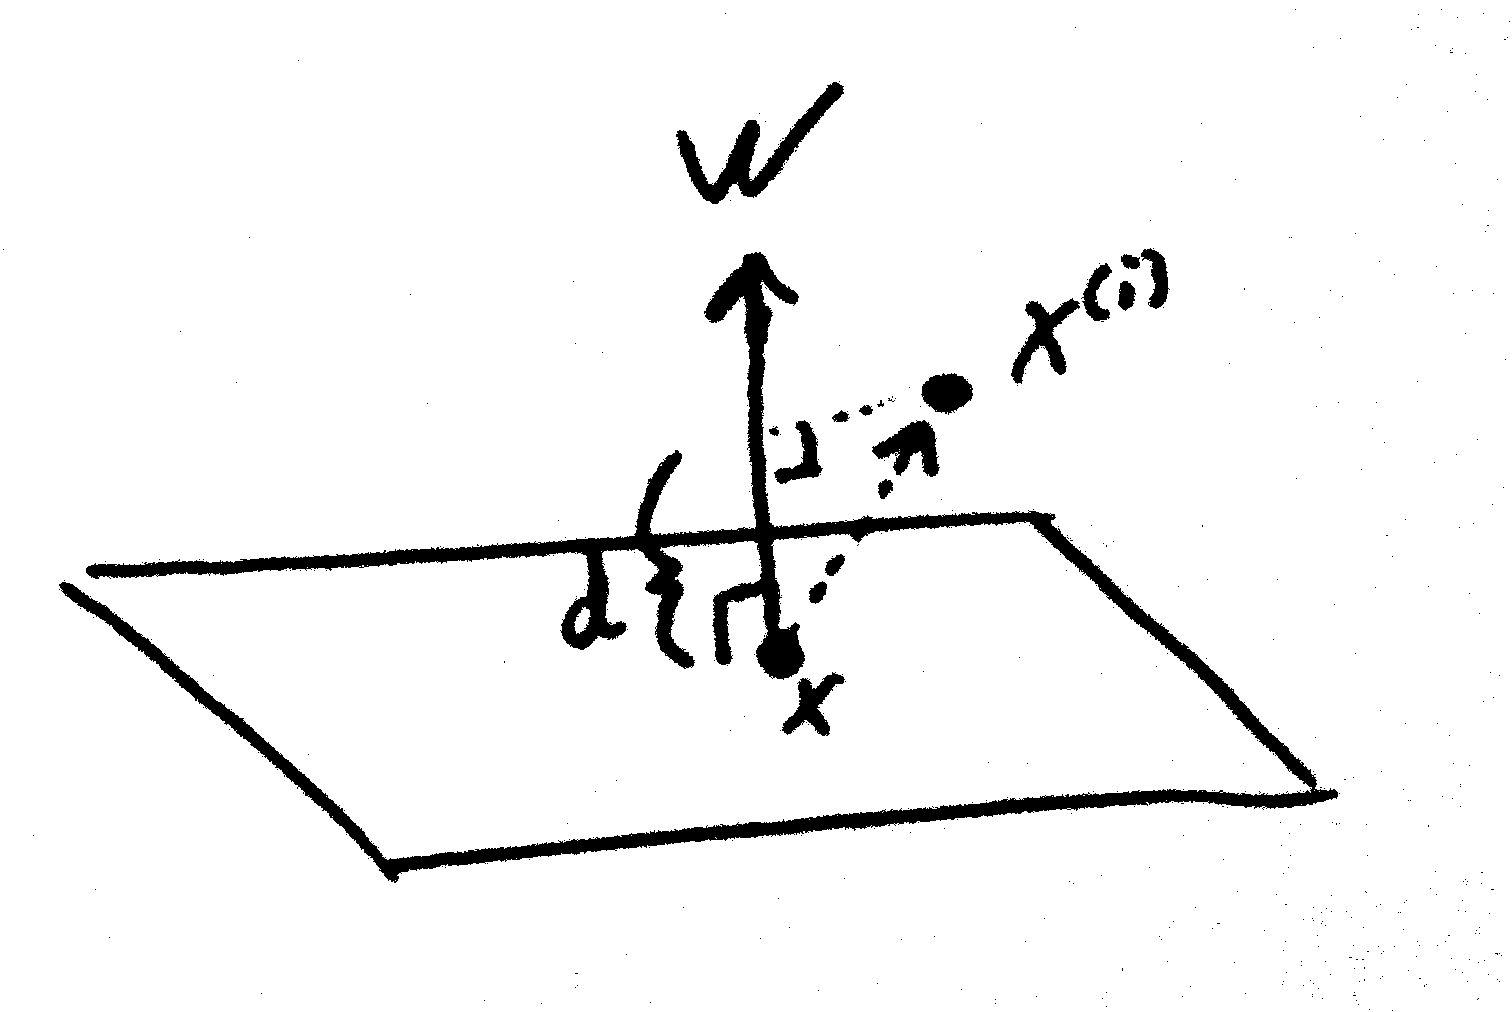
\includegraphics[width=\textwidth]{figs/distance_projection.png}
        \end{column}
    \end{columns}
\end{frame}

\begin{frame}{Maximum Margin Classifier}{First Attempt}
    \vspace{1em}
    Maximize $\frac{1}{||w||}$\\
    \vspace{2em}
    subject to:\\
    \vspace{1em}
        $ \qquad |w \cdotp x^{(i)} - b| \ge 1 $,\\
        \vspace{1em}
        \qquad \qquad for all $x^{(i)} \in D$\\
    \vspace{4em}
    \uncover<2->{
        ... but we don't know how to solve this optimization problem. Let's reformulate.
    }
\end{frame}

\begin{frame}{Maximum Margin Classifier}{Reformulated}
    \vspace{1em}
    Minimize $\frac{1}{2}||w||^2$\\
    \vspace{2em}
    subject to:\\
    \vspace{1em}
        $ \qquad y^{(i)}(w \cdotp x^{(i)} - b) \ge 1 $,\\
        \vspace{1em}
        \qquad \qquad for all $(y^{(i)}, x^{(i)}) \in D$\\
    \vspace{4em}
    \uncover<2->{
        ... plus more steps... and we eventually get a quadratic programming formulation.
    }
\end{frame}

\begin{frame}{Support Vectors}
    The maximum margin hyperplane is defined only by the points that touch the margin. These are called the ``support vectors''.
    \uncover<2->{
        \begin{center}
            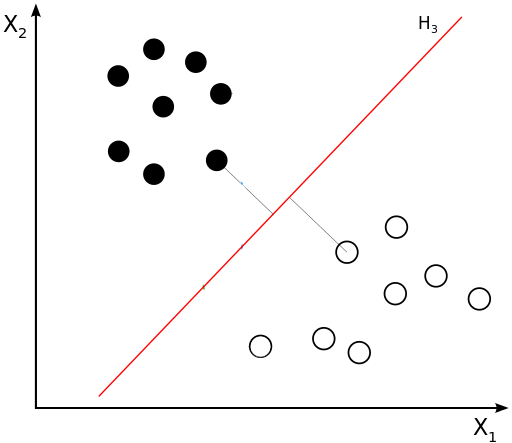
\includegraphics[width=0.5\textwidth]{figs/512px-Svm_separating_hyperplanes_2.png}
        \end{center}
    }
\end{frame}

\begin{frame}{\texttt{sklearn}'s interface}{LogisticRegression vs SVC}
    {\bf LogisticRegression:}\\
    \href{http://scikit-learn.org/stable/modules/generated/sklearn.linear_model.LogisticRegression.html}{\beamergotobutton{Link}}\\
    \vspace{1em}
    {\bf SVC:}\\
    \href{http://scikit-learn.org/stable/modules/generated/sklearn.svm.SVC.html}{\beamergotobutton{Link}}\\
    \vspace{2em}
    (end of morning lecture)
\end{frame}


\section{SVMs}

\subsection{Soft Margin}

\begin{frame}{Soft Margin Motivation}
    \vspace{1em}
    What if:
    \begin{enumerate}
        \item Your data isn't linearly separable?
        \item Your data is noisy / has outliers?
    \end{enumerate}
    \vspace{2em}
    \uncover<2->{
        Soft Margins address these problems.
    }
\end{frame}

\begin{frame}{Soft Margin}{The $C$ hyperparameter}
    An extension to Maximum Margin Classifiers adds a $C$ constant that gives the misclassification error penalty.\\
    \vspace{3em}
    \uncover<2->{
        {\bf Large $C$:} Harder margins: value classification accuracy over a large margin\\
        \vspace{1em}
    }
    \uncover<3->{
        {\bf Small $C$:} Softer margins: value a large margin over classification accuracy\\
    }
\end{frame}

\begin{frame}{Soft Margins}{Inseparable Data}
    \begin{center}
        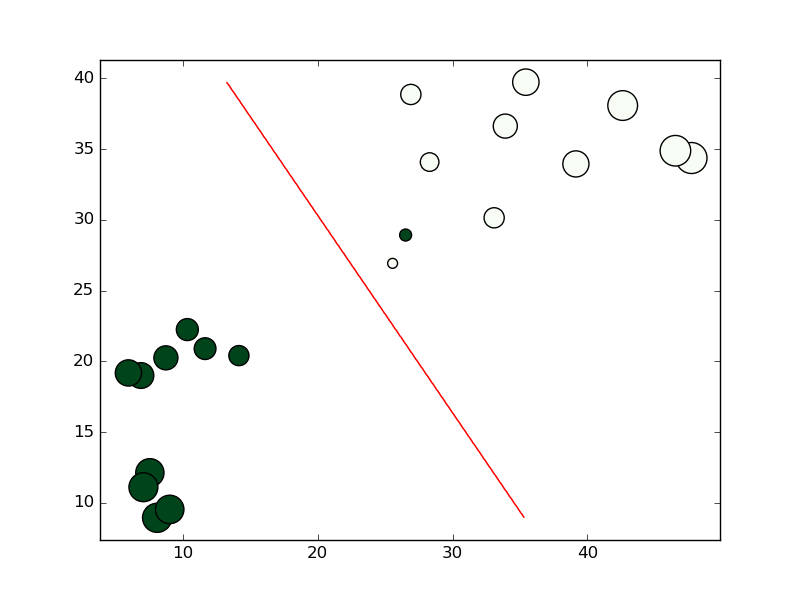
\includegraphics[width=0.7\textwidth]{figs/nonsep.png}\\
        \uncover<2->{
            Only possible with a soft margin.
        }
    \end{center}
\end{frame}

\begin{frame}{Soft Margins}{Outliers in Data}
    \begin{columns}
        \begin{column}{0.5\textwidth}
            \begin{center}
                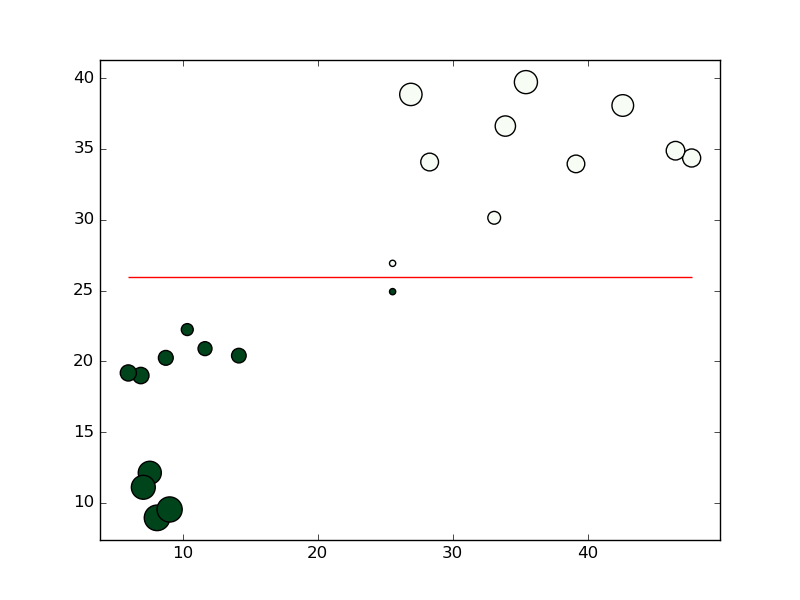
\includegraphics[width=\textwidth]{figs/outlier_hard.png}\\
                Hard Margin
            \end{center}
        \end{column}
        \begin{column}{0.5\textwidth}
            \begin{center}
                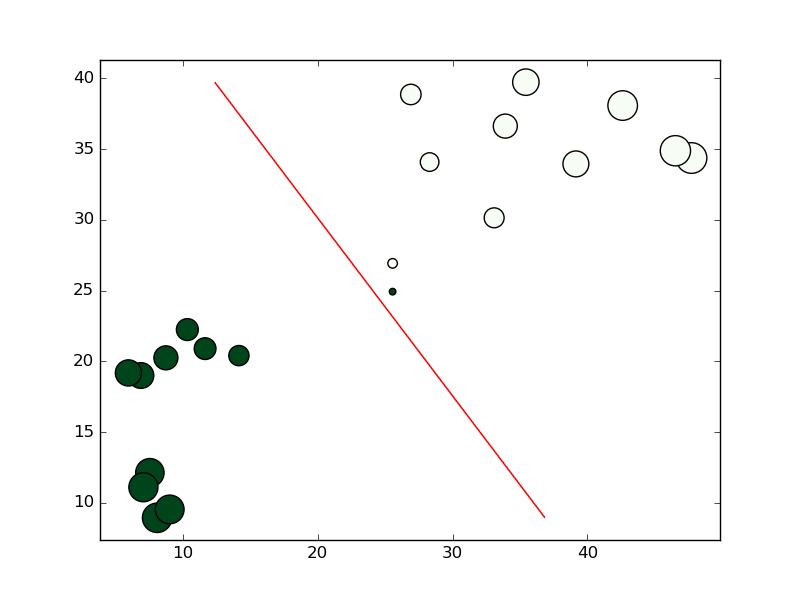
\includegraphics[width=\textwidth]{figs/outlier_soft.png}\\
                Soft Margin
            \end{center}
        \end{column}
    \end{columns}
\end{frame}

\begin{frame}[fragile]{Soft Margins}{scikit-learn code}
    \begin{lstlisting}
    from sklearn.svm import SVC
    ...
    svc = SVC(C=1.0, kernel='linear')
    svc.fit(x, y)
    \end{lstlisting}
    \vspace{2em}
    SVC supports the $C$ parameter as the soft-margin hyperparameter.
\end{frame}

\subsection{Kernels}

\begin{frame}{The ``Kernel Trick''}{The idea...}
    Idea: If data is inseparable in its input space, maybe it will be separable in a higher-dimensional space.
    \begin{center}
        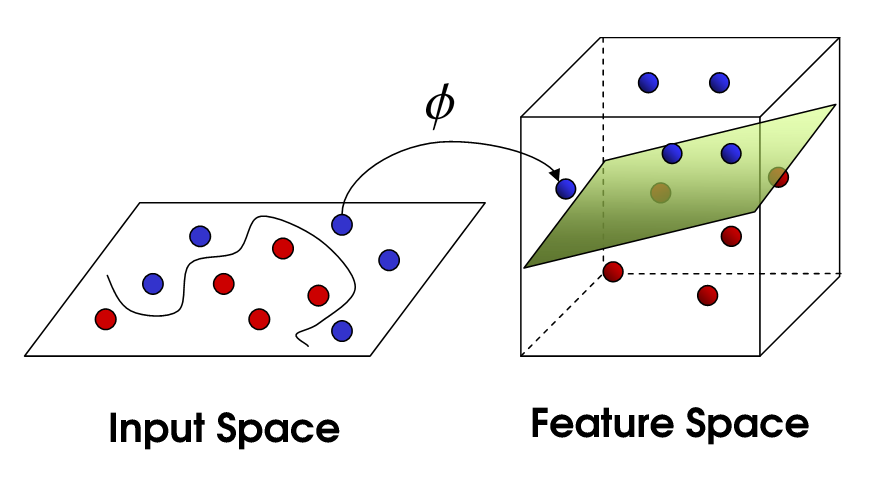
\includegraphics[width=0.7\textwidth]{figs/kernel.png}
    \end{center}
    \footnotetext[1]{Unknown source}
\end{frame}

\begin{frame}{The ``Kernel Trick''}{Back to the math...}
    \vspace{1em}
    In our optimization problem to maximize the margin, we eventually end up optimizing a vector alpha $\alpha^{(i)}, i \in [1, m]$ in the following equation:
    \vspace{1em}
    \uncover<2->{
        $$\mathcal{L}(\alpha) = \sum_{i=1}^m \alpha^{(i)} - \frac{1}{2} \sum_{i=1}^m \sum_{j=1}^m y^{(i)} y^{(j)} \alpha^{(i)} \alpha^{(j)} ( {\color{blue} x^{(i)} \cdotp x^{(j)} } )$$
        \vspace{1em}
    }
    \uncover<3->{
        $$\mathcal{L}(\alpha) = \sum_{i=1}^m \alpha^{(i)} - \frac{1}{2} \sum_{i=1}^m \sum_{j=1}^m y^{(i)} y^{(j)} \alpha^{(i)} \alpha^{(j)} ( {\color{blue} \phi(x^{(i)}) \cdotp \phi(x^{(j)}) } )$$
    }
\end{frame}

\begin{frame}{The ``Kernel Trick''}{Creating a kernel...}
    \vspace{1em}
    $$\phi(x^{(i)}) \cdotp \phi(x^{(j)}) \in \mathbb{R}$$
    ... this is just a real number.\\
    \vspace{3em}
    \uncover<2->{
        What if we never applied $\phi$ and we never took the dot product, but we instead replaced this whole thing with a ``kernel function''.
    }
    \uncover<3->{
        $$K(x^{(i)}, x^{(j)}) = \phi(x^{(i)}) \cdotp \phi(x^{(j)}) \in \mathbb{R}$$
    }
\end{frame}

\begin{frame}{The ``Kernel Trick''}{Why is this so cool?}
    \begin{itemize}
        \item Saves some computation. We never need to compute $\phi$.
        \item Opens new possibilities. A kernel can operate in infinite dimensions!
    \end{itemize}
    \vspace{2em}
    \uncover<2->{
        You can use any $K(x^{(i)}, x^{(j)})$ as long as there {\bf exists} some $\phi$ such that
            $$K(x^{(i)}, x^{(j)}) = \phi(x^{(i)}) \cdotp \phi(x^{(j)})$$
        ... but you don't have to know what $\phi$ actually {\bf is}!
    }
\end{frame}

\begin{frame}{The Polynomial Kernel}
    \vspace{1em}
    $$K(x^{(i)}, x^{(j)}) = (1 + x^{(i)} \cdotp x^{(j)})^d$$
    \begin{itemize}
        \item<2-> equivalent to the dot product in the $d$-order $\phi$ space
        \item<3-> requires an extra hyper-parameter, $d$, for ``degree''
    \end{itemize}
    \vspace{2em}
\end{frame}

\begin{frame}{The Polynomial Kernel}{Example}
    \begin{columns}
        \begin{column}{0.33\textwidth}
            \begin{center}
                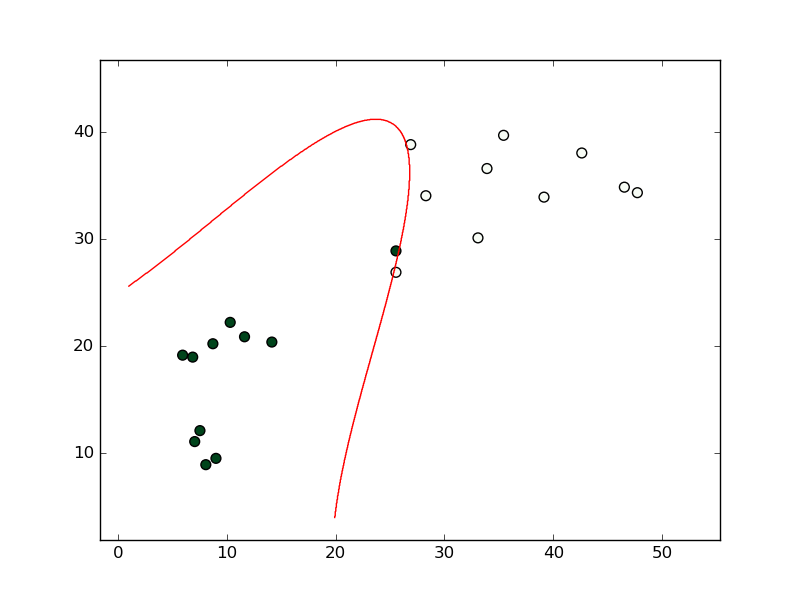
\includegraphics[width=\textwidth]{figs/poly_d3.png}
            \end{center}
            svc = SVC(C=10000.0, kernel='poly', degree=3)
        \end{column}
        \begin{column}{0.33\textwidth}
            \begin{center}
                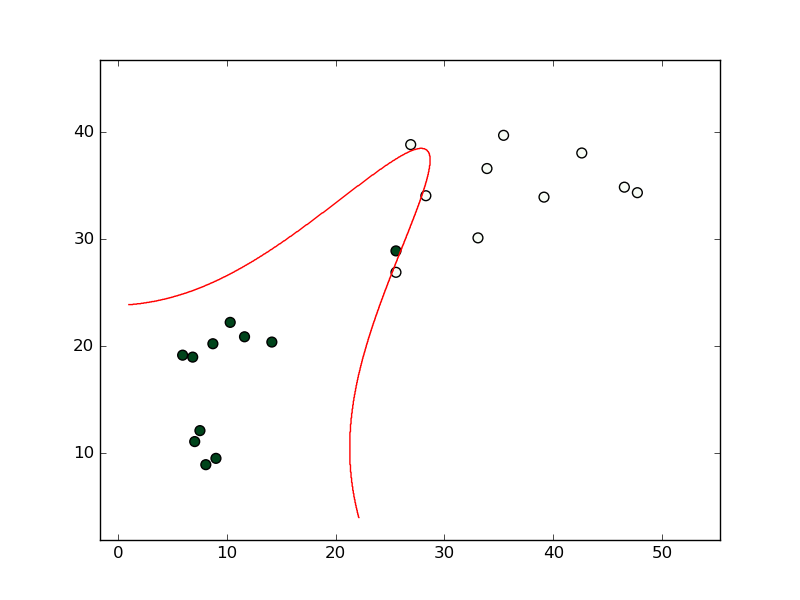
\includegraphics[width=\textwidth]{figs/poly_d5.png}
            \end{center}
            svc = SVC(C=10000.0, kernel='poly', degree=5)
        \end{column}
        \begin{column}{0.33\textwidth}
            \begin{center}
                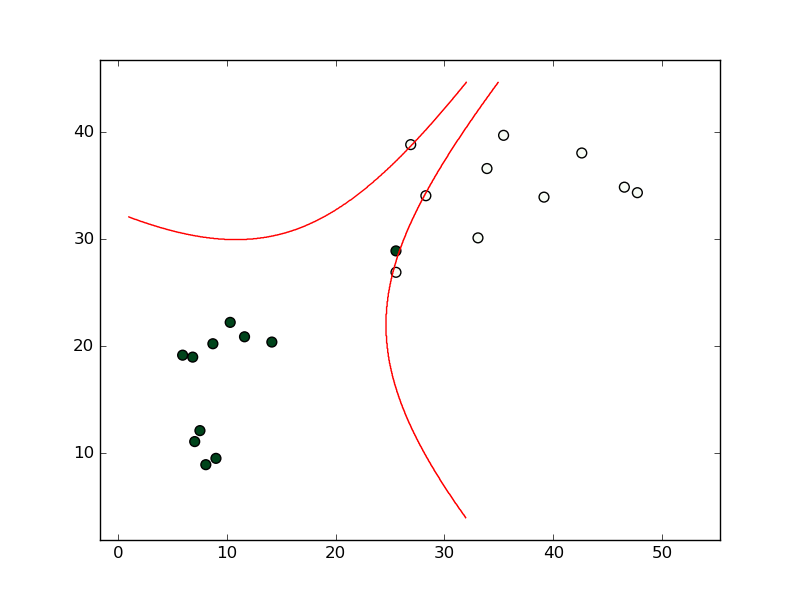
\includegraphics[width=\textwidth]{figs/poly_d10.png}
            \end{center}
            svc = SVC(C=10000.0, kernel='poly', degree=10)
        \end{column}
    \end{columns}
\end{frame}

\begin{frame}{The RBF Kernel}{(Radial Basis Function)}
    \vspace{1em}
    $$K(x^{(i)}, x^{(j)}) = \exp{( -\gamma || x^{(i)} - x^{(j)} ||^2 )}$$
    \begin{itemize}
        \item<2-> equivalent to the dot product in the Hilbert space of infinite dimensions
        \item<3-> requires an extra hyper-parameter, $\gamma$, ``gamma''
    \end{itemize}
    \vspace{2em}
\end{frame}

\begin{frame}{The RBF Kernel}{Examples}
    \begin{columns}
        \begin{column}{0.5\textwidth}
            \begin{center}
                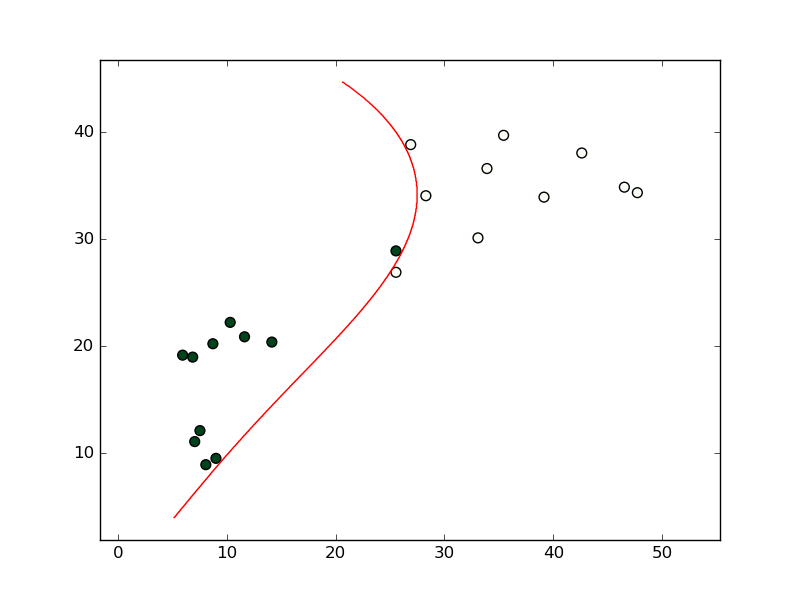
\includegraphics[width=\textwidth]{figs/gamma_1e-3.png}
            \end{center}
            svc = SVC(C=10000.0, kernel='rbf', gamma=0.001)
        \end{column}
        \begin{column}{0.5\textwidth}
            \begin{center}
                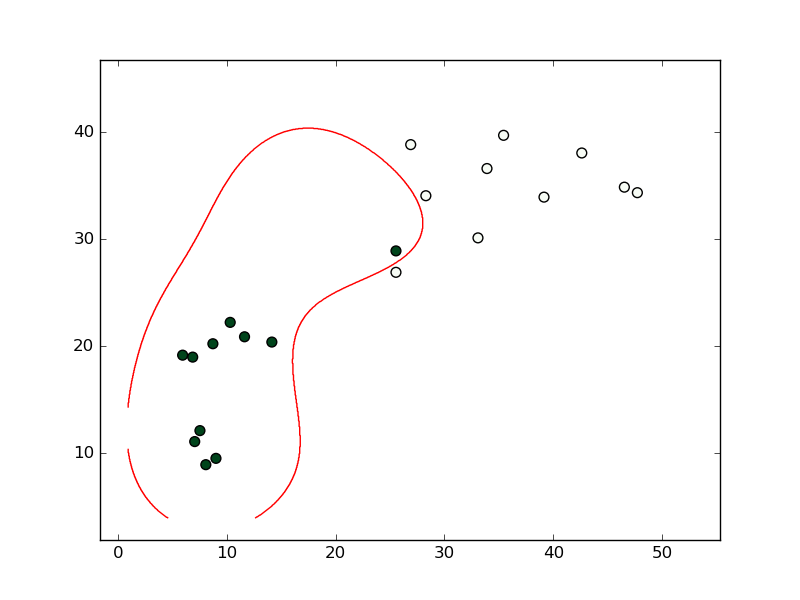
\includegraphics[width=\textwidth]{figs/gamma_1e-2.png}
            \end{center}
            svc = SVC(C=10000.0, kernel='rbf', gamma=0.01)
        \end{column}
    \end{columns}
\end{frame}

\begin{frame}{The RBF Kernel}{More Examples}
    \begin{columns}
        \begin{column}{0.5\textwidth}
            \begin{center}
                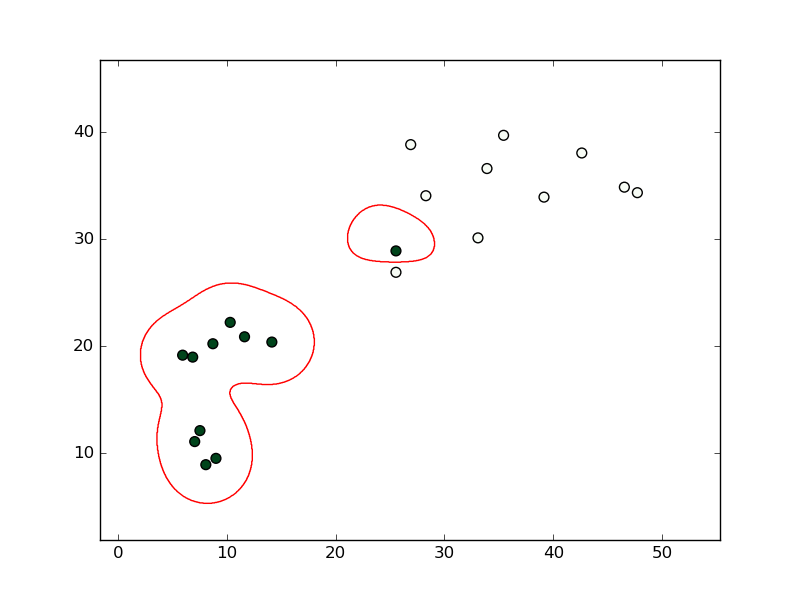
\includegraphics[width=\textwidth]{figs/gamma_1e-1.png}
            \end{center}
            svc = SVC(C=10000.0, kernel='rbf', gamma=0.1)
        \end{column}
        \begin{column}{0.5\textwidth}
            \begin{center}
                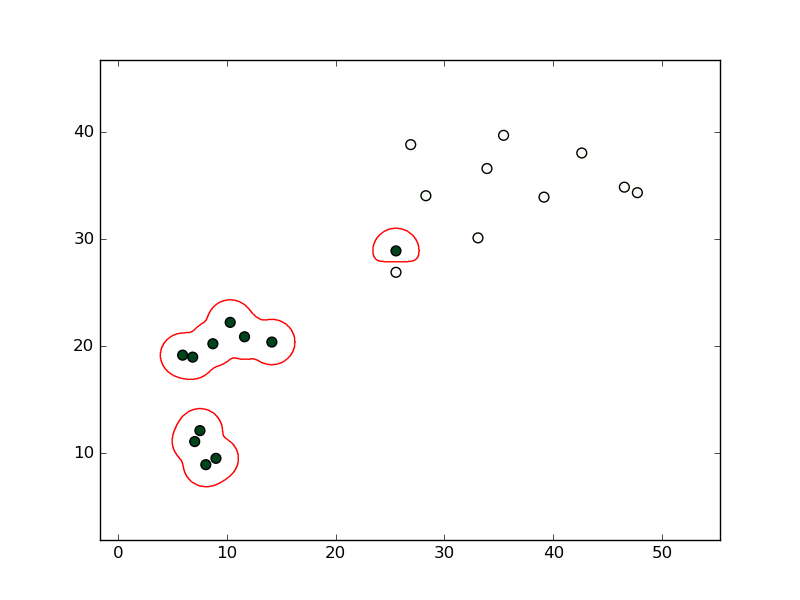
\includegraphics[width=\textwidth]{figs/gamma_1.png}
            \end{center}
            svc = SVC(C=10000.0, kernel='rbf', gamma=1.0)
        \end{column}
    \end{columns}
\end{frame}

\begin{frame}{Bias-Variance tradeoff}{Explanation}
    \begin{columns}
        \begin{column}{0.5\textwidth}
            {\bf Bias} \\
            \vspace{1em}
            \uncover<2->{
                A high-``bias'' model makes many assumptions and prefers to solve problems a certain way.\\
            }
            \vspace{1em}
            \uncover<3->{
                E.g. A linear SVM looks for dividing hyperplanes in the input space {\em only}.\\
            }
            \vspace{1em}
            \uncover<4->{
                For complex data, high-bias models often {\em underfit} the data.
            }
        \end{column}
        \begin{column}{0.5\textwidth}
            {\bf Variance} \\
            \vspace{1em}
            \uncover<5->{
                A high-``variance'' model makes fewer assumptions and has more representational power.\\
            }
            \vspace{1em}
            \uncover<6->{
                E.g. An RBF SVM looks for dividing hyperplanes in an infinite-dimensional space.\\
            }
            \vspace{1em}
            \uncover<7->{
                For simple data, high-variance models often {\em overfit} the data.
            }
        \end{column}
    \end{columns}
\end{frame}

\begin{frame}{Bias-Variance tradeoff}{Example}
    \begin{columns}
        \begin{column}{0.5\textwidth}
            \begin{center}
                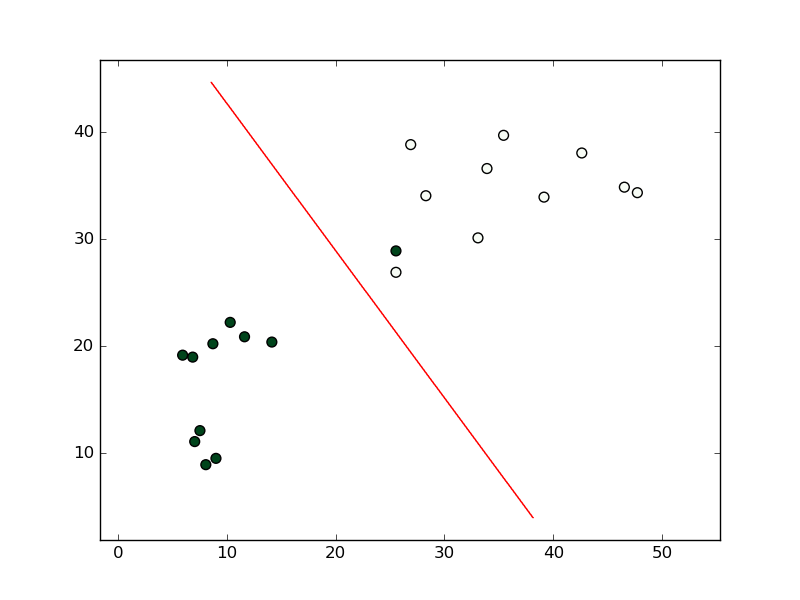
\includegraphics[width=0.8\textwidth]{figs/basic_linear.png}
            \end{center}
            svc = SVC(C=0.01, kernel="linear")
        \end{column}
        \begin{column}{0.5\textwidth}
            \begin{center}
                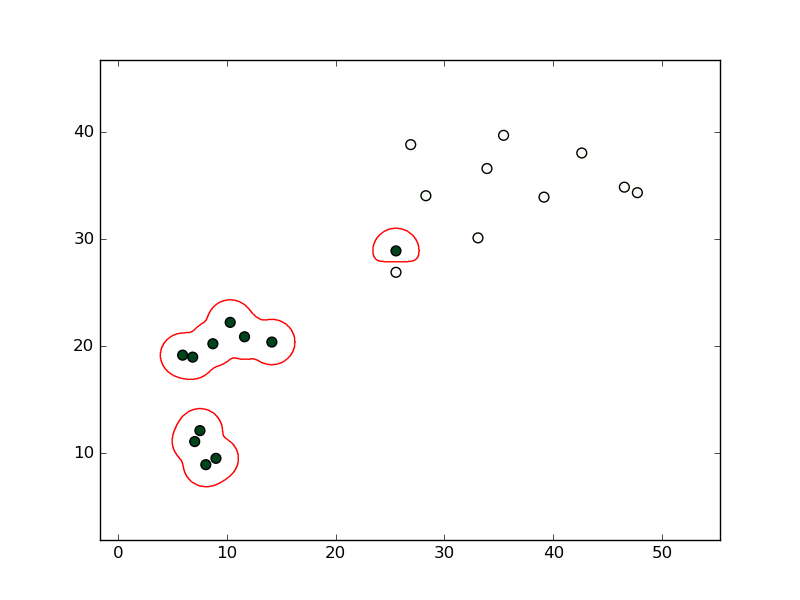
\includegraphics[width=0.8\textwidth]{figs/gamma_1.png}
            \end{center}
            svc = SVC(C=10000.0, kernel='rbf', gamma=1.0)
        \end{column}
    \end{columns}
    \vspace{1em}
    \uncover<2->{
        \begin{center}
            \alert{Which is a better fit for this dataset?}
        \end{center}
    }
\end{frame}

\subsection{Misc Topics}

\begin{frame}{SVMs vs Logistic Regression}{(some rules of thumb)}
    \begin{enumerate}
        \item Logistic Regression maximizes the {\em Binomial Log Likelihood} function.
        \item SVMs maximize the {\em margin}.
        \item When classes are nearly separable, SVMs tends to do better than Logistic Regression.
        \item Otherwise, Logistic Regression (with Ridge) and SVMs are similar.
        \item However, if you want to estimate probabilities, Logistic Regression is the better choice.
        \item With kernels, SVMs work well. Logistic Regression works fine with kernels but can get computationally too expensive.
    \end{enumerate}
\end{frame}

\begin{frame}{Grid Search}{Hyperparameter Tuning}
    \begin{columns}
        \begin{column}{0.4\textwidth}
            \uncover<2->{
                Let's find $C$ and $gamma$ by searching through values we expect might work well.\\
                \vspace{1em}
            }
            \uncover<3->{
                \alert{Use cross-validation accuracy to determine which values are best.}\\
            }
        \end{column}
        \begin{column}{0.6\textwidth}
            \begin{center}
                \uncover<4->{
                    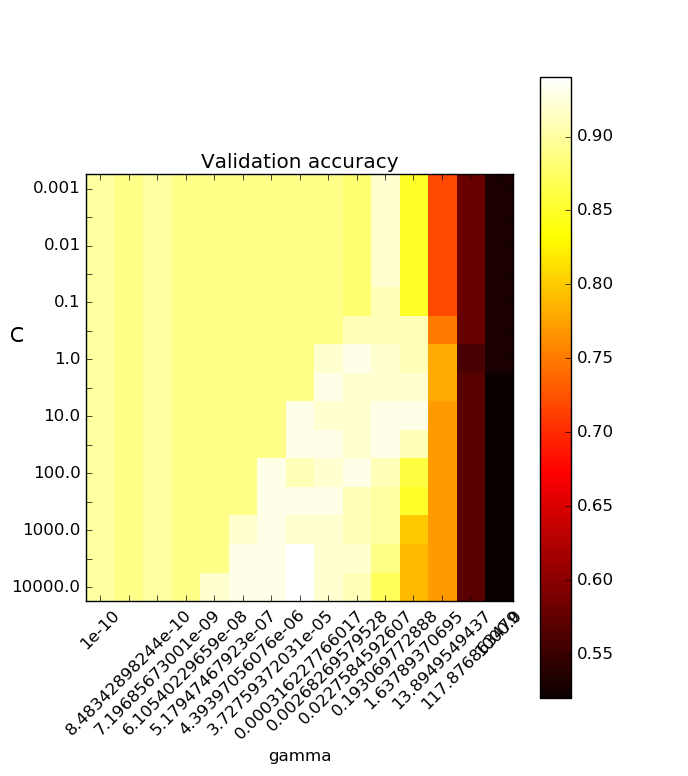
\includegraphics[width=0.9\textwidth]{figs/grid_search.png}\\
                }
            \end{center}
%           Using:
%           \begin{itemize}
%               \item \texttt{GridSearchCV},
%               \item \texttt{non\_sep.csv},
%               \item \texttt{RBF Kernel}.
%           \end{itemize}
%           Solution: \{'C': 3162.2776601683795, 'gamma': 0.00031622776601683794\}\\
%           Best Accuracy: 0.94
        \end{column}
    \end{columns}
\end{frame}

\begin{frame}[fragile]{Grid Search}{code}
    \begin{verbatim}
svc_rbf = SVC(kernel='rbf')

param_space = {'C':     np.logspace(-3, 4, 15),
               'gamma': np.logspace(-10, 3, 15)}

grid_search = GridSearchCV(svc_rbf, param_space,
                           scoring='accuracy', cv=10)
grid_search.fit(x, y)

print grid_search.grid_scores_
print grid_search.best_params_
print grid_search.best_score_
print grid_search.best_estimator_
    \end{verbatim}
\end{frame}


\end{document}
